\section{Conversor buck-boost}\label{sec:conversor}

Arquivos: \arq{conversor/parametros_conversor.m}, \arq{conversor_ideal.m}, \arq{conversor_medio_rhs.m},
\arq{equilibrio_conversor.m}, \arq{verifica_ccm.m}, \arq{sim_chaveado.m}, \arq{sim_medio_aberta.m}.
O conversor \'e quem imp\~oe ao painel a tens\~ao de opera\c{c}\~ao. Sem ele n\~ao h\'a como o MPPT
``escolher'' o ponto da curva.

\subsection{Como funciona o buck-boost inversor}

O conversor tem uma chave (MOSFET), um indutor $L$, um diodo Schottky e um capacitor $C$ na
entrada, em paralelo com o painel. Em cada per\'iodo $T_s=1/f_s$:

\begin{itemize}
\item \textbf{Chave ligada} (fra\c{c}\~ao $d$ do per\'iodo, a \emph{raz\~ao c\'iclica}): o indutor fica
 ligado ao painel e \emph{carrega}; a corrente $i_L$ sobe.
\item \textbf{Chave desligada} (fra\c{c}\~ao $1-d$): o indutor \'e desligado do painel e
 \emph{descarrega} na bateria pelo diodo; $i_L$ cai.
\end{itemize}

\begin{figure}[htbp]
\centering
\begin{circuitikz}[scale=0.9,transform shape]
  \draw (0,0) to[isource,l_=Painel] (0,3) -- (1.8,3);
  \draw (1.8,3) to[C,l=$C$] (1.8,0);
  \draw (1.8,3) to[cspst,l=$S$] (4.3,3);
  \draw (4.3,3) to[L,l=$L$] (4.3,0);
  \draw (4.3,3) -- (5,3) to[D,l_=$D$] (7,3) -- (7,2.4);
  \draw (7,2.4) to[battery2,l=$V_{bat}$] (7,0.6) -- (7,0);
  \draw (0,0) -- (7,0);
  \node[font=\scriptsize] at (7.45,0.45) {$+$};
  \node[font=\scriptsize] at (7.45,2.55) {$-$};
  \node[font=\scriptsize,gray,anchor=west] at (2.2,-0.7) {Polaridade invertida: a bateria \'e carregada pela corrente do diodo.};
\end{circuitikz}
\caption{Conversor buck-boost inversor, entre o painel (com o capacitor de entrada $C$) e a bateria.}
\label{fig:circuito_conv}
\end{figure}

\begin{figure}[htbp]
\centering
\begin{tikzpicture}
  \node[ctrl,minimum width=6.4cm,minimum height=2.1cm,align=left] (on) at (0,0)
    {\textbf{Chave ligada, fra\c{c}\~ao $d$}\\[2pt]{\scriptsize $L\,\dfrac{di_L}{dt}=\vpv-i_L(r_L+R_{on})$}\\[4pt]{\scriptsize $C\,\dfrac{d\vpv}{dt}=\ipv-i_L$}};
  \node[dest,minimum width=6.4cm,minimum height=2.1cm,align=left] (off) at (7.4,0)
    {\textbf{Chave desligada, fra\c{c}\~ao $1-d$}\\[2pt]{\scriptsize $L\,\dfrac{di_L}{dt}=-(V_{bat}+V_F)-i_L(r_L+R_D)$}\\[4pt]{\scriptsize $C\,\dfrac{d\vpv}{dt}=\ipv$}};
  \draw[seta,bend left=18] (on.north east) to node[rot,above]{$d\,T_s$} (off.north west);
  \draw[seta,bend left=18] (off.south west) to node[rot,below]{$(1-d)\,T_s$} (on.south east);
\end{tikzpicture}
\caption{As duas topologias que se alternam a cada per\'iodo de chaveamento.}
\label{fig:duas_topologias}
\end{figure}

No regime permanente a tens\~ao m\'edia no indutor \'e zero (o fluxo n\~ao pode crescer sem limite).
Sem perdas isso d\'a $d\,\vpv=(1-d)\,V_{bat}$, ou
\begin{equation}\label{eq:d_ideal}
d=\frac{V_{bat}}{V_{bat}+\vpv},\qquad i_L=\frac{\ipv}{d}.
\end{equation}
A raz\~ao c\'iclica \'e a ``alavanca'' do MPPT: mudar $d$ muda $\vpv$. Com $V_{bat}=12$\,V e
$\vpv=19{,}57$\,V (MPP de STC), $d=0{,}38<0{,}5$: o conversor trabalha como buck. Se o pico global
cai para 7\,V, $d=0{,}63$ e trabalha como boost.

\subsection{Dimensionamento}

\codigointeiro{conversor/parametros_conversor.m}{$L$ e $C$ pelo ripple no MPP de STC, perdas t\'ipicas.}{lst:paramconv}

\begin{logica}
\begin{enumerate}
\item Ponto de projeto: MPP de STC (\texttt{curva\_pv} com $G=1000$ em todos os subm\'odulos).
\item $D=V_{bat}/(V_{bat}+V_{mp})\approx0{,}380$ e $I_L=I_{mp}/D\approx21{,}6$\,A (eq.~\ref{eq:d_ideal}).
\item \textbf{Indutor}: com a chave ligada, $\Delta i=\vpv D T_s/L$. Impondo ripple de 30\,\% de $I_L$:
 $L=V_{mp}D/(0{,}30\,I_Lf_s)\approx57\,\mu$H.
\item \textbf{Capacitor}: com a chave ligada o indutor puxa $i_L$ do capacitor; a carga trocada por ciclo \'e
 $I_LD(1-D)T_s$. Com ripple de tens\~ao de 1\,\%: $C=I_LD(1-D)/(0{,}01\,V_{mp}f_s)\approx1{,}3$\,mF.
\item Perdas de cat\'alogo: $r_L=20$\,m$\Omega$, $R_{on}=18$\,m$\Omega$, $V_F=0{,}45$\,V, $R_D=10$\,m$\Omega$,
 $t_r+t_f=100$\,ns; limites $d\in[0{,}02;\,0{,}95]$; atraso do PWM $1{,}5T_s=75\,\mu$s.
\end{enumerate}
\end{logica}

O ripple real fica em $\sim$34 a 35\,\%, n\~ao 30\,\%, porque o $d$ real (com perdas) \'e maior que o ideal usado
no projeto. A MOSFET \'e de classe 60\,V porque a chave v\^e $\vpv+V_{bat}\approx37$\,V. As perdas s\~ao t\'ipicas de
cat\'alogo, e o E7 mede o efeito delas (com e sem perdas), ent\~ao a conclus\~ao n\~ao depende dos valores exatos.

\subsection{Tr\^es modelos do mesmo conversor}

\begin{center}\small
\begin{tabularx}{\textwidth}{@{}lXX@{}}
\toprule
Modelo & O que faz & Quando usar \\ \midrule
\textbf{Ideal} (\arq{conversor_ideal}) & Zera todas as perdas & Compara\c{c}\~ao: ``quanto as perdas custam?'' \\
\textbf{M\'edio com perdas} (\arq{conversor_medio_rhs}) & M\'edia ponderada pelo tempo das duas topologias; sem ripple & Simula\c{c}\~oes longas (dia inteiro) \\
\textbf{Chaveado} (\arq{sim_chaveado}) & Alterna as topologias de fato, 200 passos por per\'iodo & S\'o para validar o m\'edio, em janelas de ms \\
\bottomrule
\end{tabularx}
\end{center}

\subsubsection{Modelo m\'edio}

\begin{equation}\label{eq:medio}
C\frac{d\vpv}{dt}=\ipv-d\,i_L,\qquad
L\frac{di_L}{dt}=d\,\vpv-(1-d)(V_{bat}+V_F)-i_L\big(r_L+d\,R_{on}+(1-d)R_D\big)
\end{equation}

\codigointeiro{conversor/conversor_medio_rhs.m}{lado direito do modelo m\'edio.}{lst:medio}

\begin{logica}
Cada termo da eq.~\eqref{eq:medio} \'e a m\'edia ponderada pelo tempo das duas topologias da
Figura~\ref{fig:duas_topologias}: o que ocorre com a chave ligada multiplica-se por \texttt{d}; o que ocorre
com ela desligada, por \texttt{(1-d)}. O capacitor s\'o \'e descarregado pelo indutor durante a fra\c{c}\~ao
\texttt{d}.
\end{logica}

\subsubsection{Modelo chaveado}

\codigo{conversor/sim_chaveado.m}{44}{85}{o la\c{c}o de Euler com 200 passos por per\'iodo.}{lst:chaveado}

\begin{logica}
\begin{enumerate}
\item A cada passo guarda-se o estado \emph{antes} de avan\c{c}ar; \texttt{j} \'e o \'indice do passo dentro do per\'iodo.
\item \textbf{PWM real:} $d$ \'e amostrado no in\'icio de cada per\'iodo (\texttt{j == 0}) e fica fixo at\'e o pr\'oximo.
\item \texttt{f} \'e a fra\c{c}\~ao do passo com a chave ligada: 1 antes de $d\cdot200$, 0 depois, e fracion\'ario no passo da
 comuta\c{c}\~ao. Sem isso o $d$ efetivo erraria em at\'e $1/200$.
\item O painel \'e resolvido por Newton (com \emph{warm start}) na tens\~ao atual do capacitor.
\item As derivadas das duas topologias s\~ao combinadas por \texttt{f} e o estado avan\c{c}a por Euler.
\item O diodo bloqueia corrente reversa: \texttt{iL = max(..., 0)}. Quando $i_L$ chega a zero, entra-se em DCM.
\end{enumerate}
A condi\c{c}\~ao inicial parte do instante em que a chave liga ($i_L$ no vale, $\vpv$ no pico): partir da m\'edia
deslocaria o resultado em meio ripple ($\sim$17\,\% em STC) e excitaria uma oscila\c{c}\~ao LC que n\~ao existe no modelo m\'edio.
\end{logica}

\subsection{O equil\'ibrio com perdas}

Dado $(\vpv,\ipv)$, \arq{equilibrio_conversor} acha $d$ e a efici\^encia. Em regime, $d\vpv/dt=0$ d\'a
$i_L=\ipv/d$. Substituindo em $di_L/dt=0$ e multiplicando por $d$, chega-se a uma equa\c{c}\~ao do 2.\textordmasculine\ grau:
\begin{equation}\label{eq:quadratica}
(\vpv+V_t)\,d^2-\big(V_t+\ipv(R_{on}-R_D)\big)\,d-\ipv(r_L+R_D)=0,\qquad V_t=V_{bat}+V_F .
\end{equation}
O coeficiente de $d^2$ \'e positivo e o termo constante \'e negativo: o produto das ra\'izes \'e negativo e h\'a
\textbf{exatamente uma raiz positiva}. N\~ao precisa de \texttt{fzero}.

\codigointeiro{conversor/equilibrio_conversor.m}{raiz da quadr\'atica, perdas e efici\^encia.}{lst:equilibrio}

\begin{logica}
\begin{enumerate}
\item Se $\ipv\le0$ (noite): sem transfer\^encia, devolve tudo zerado e \texttt{viavel = false}.
\item \texttt{a}, \texttt{b}, \texttt{c} s\~ao os coeficientes de (\ref{eq:quadratica}); \texttt{d} \'e a raiz positiva.
\item Se $d$ sai de $[D_{min},D_{max}]$ o controlador n\~ao alcan\c{c}a o ponto: tamb\'em sem transfer\^encia.
\item \textbf{Perda de condu\c{c}\~ao:} $P_{cond}=i_L^2(r_L+dR_{on}+(1-d)R_D)+(1-d)i_LV_F$.
\item \textbf{Perda de chaveamento:} $P_{sw}=\tfrac12(\vpv+V_{bat})\,i_L\,(t_r+t_f)\,f_s$ (sobreposi\c{c}\~ao tens\~ao $\times$ corrente).
\item \textbf{Pot\^encia na bateria:} $P_{out}=(1-d)\,i_LV_{bat}-P_{sw}$; $\eta=P_{out}/(\vpv\ipv)$.
\end{enumerate}
$P_{sw}$ entra s\'o no balan\c{c}o de pot\^encia, n\~ao na EDO m\'edia ($<1$\,\% em STC).
\end{logica}

\subsection{CCM e DCM}

\codigointeiro{conversor/verifica_ccm.m}{teste de condu\c{c}\~ao cont\'inua.}{lst:ccm}

O ripple pico a pico \'e $\vpv\,d/(L f_s)$ e a condu\c{c}\~ao \'e cont\'inua (\textbf{CCM}) se $i_L>\text{ripple}/2$.
Em baixa luz (50\,W/m$^2$) a corrente m\'edia ($\sim$1\,A) \'e menor que meio ripple ($\sim$3\,A): o conversor entra em
\textbf{condu\c{c}\~ao descont\'inua (DCM)}. Ali o modelo m\'edio de CCM deixa de valer e a efici\^encia calculada fica
\emph{otimista}, pois as perdas de condu\c{c}\~ao dependem da corrente RMS, bem maior que a m\'edia.

\subsection{Valida\c{c}\~ao chaveado $\times$ m\'edio (E3)}

O experimento aplica um degrau de $+0{,}02$ em $d$, em $t=2$\,ms, partindo do MPP, e compara o modelo m\'edio com a m\'edia
m\'ovel de um per\'iodo do chaveado.

\begin{itemize}
\item \textbf{Em STC (CCM):} o m\'edio segue o chaveado. O teste de regress\~ao exige desvio m\'aximo $<0{,}5$\,\% na tens\~ao e
 $<1{,}5$\,\% na corrente, e ripple de $i_L$ dentro de 15\,\% do valor te\'orico.
\item \textbf{Em 50\,W/m$^2$ (DCM):} as curvas se separam, e isso \'e o resultado esperado. Em DCM a energia puxada por
 ciclo \'e fixada por $(\vpv dT_s)^2/(2L)$, muito maior que a pot\^encia do painel nessa luz; o m\'edio chega a dar
 $i_L<0$, imposs\'ivel fisicamente. O experimento mostra o \emph{limite de validade} do modelo m\'edio.
\end{itemize}

\begin{figure}[htbp]
\centering
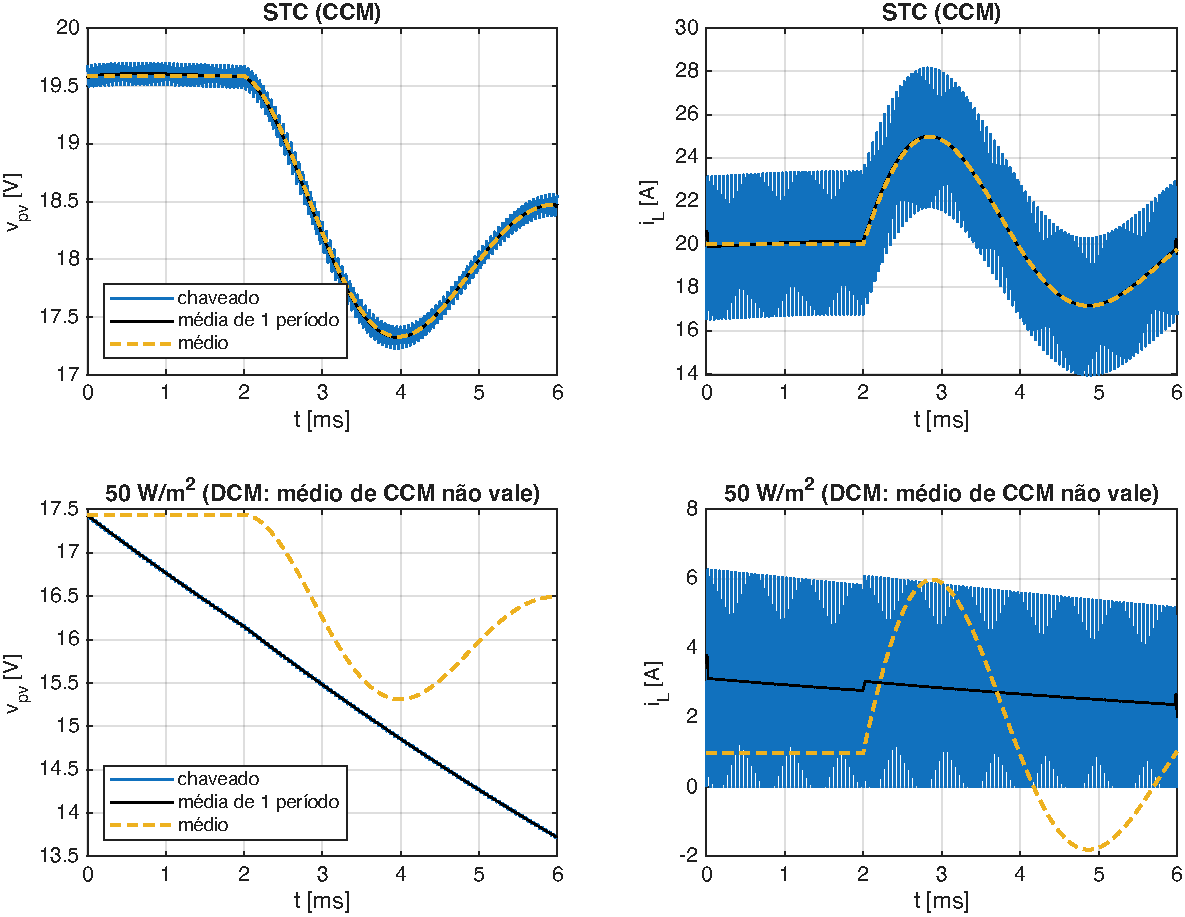
\includegraphics[width=0.9\linewidth]{e3_chaveado_medio.pdf}
\caption{E3. Modelo chaveado (com ripple), m\'edia m\'ovel de um per\'iodo e modelo m\'edio. Em cima, STC (CCM); embaixo,
50\,W/m$^2$ (DCM).}
\label{fig:e3}
\end{figure}

\subsection{Malha aberta com DAE (\texttt{sim\_medio\_aberta})}

Integra o modelo m\'edio mais o painel como DAE (equa\c{c}\~oes diferenciais e alg\'ebricas) com \texttt{ode15s} e matriz de
massa $M=\mathrm{diag}(1,1,0,\dots,0)$: as duas primeiras linhas s\~ao EDOs ($\vpv$ e $i_L$) e as demais s\~ao as
restri\c{c}\~oes alg\'ebricas do painel. O jacobiano anal\'itico \'e obrigat\'orio, pois com diferen\c{c}as finitas a
exponencial do bypass faz o \texttt{ode15s} falhar. Ela s\'o \'e usada no E3; a malha fechada usa a EDO reduzida
(Cap\'itulo~\ref{sec:sim}), porque a DAE falhou em 9 de 36 casos quando o MPPT dava degraus grandes.
